% Credits are indicated where needed. The general idea is based on a template by Vel (vel@LaTeXTemplates.com) and Frits Wenneker.

\documentclass[11pt, a4paper]{article} % General settings in the beginning (defines the document class of your paper)
% 11pt = is the font size
% A4 is the paper size
% “article” is your document class

%----------------------------------------------------------------------------------------
% Packages
%----------------------------------------------------------------------------------------

% Necessary
\usepackage[german,english]{babel} % English and German language 
\usepackage{booktabs} % Horizontal rules in tables 
% For generating tables, use “LaTeX” online generator (https://www.tablesgenerator.com)
\usepackage{comment} % Necessary to comment several paragraphs at once
\usepackage[utf8]{inputenc} % Required for international characters
\usepackage[T1]{fontenc} % Required for output font encoding for international characters

% Might be helpful
\usepackage{amsmath,amsfonts,amsthm} % Math packages which might be useful for equations
\usepackage{tikz} % For tikz figures (to draw arrow diagrams, see a guide how to use them)
\usepackage{tikz-cd}
\usepackage{hyperref}

\usepackage{listings}

\usetikzlibrary{positioning,arrows} % Adding libraries for arrows
\usetikzlibrary{decorations.pathreplacing} % Adding libraries for decorations and paths
\usepackage{tikzsymbols} % For amazing symbols ;) https://mirror.hmc.edu/ctan/graphics/pgf/contrib/tikzsymbols/tikzsymbols.pdf 
\usepackage{blindtext} % To add some blind text in your paper
\theoremstyle{definition}
\newtheorem{definition}{Definition}[section]

\newcommand\tab[1][1cm]{\hspace*{#1}}
\newcommand\ftab[1][5cm]{\hspace*{#1}}
\newcommand\ttab[1][2cm]{\hspace*{#1}}
\newcommand\tsp[1][0.2cm]{\hspace*{#1}}


\graphicspath{ {images/} }

\newtheorem*{theorem}{Theorem}
\newtheorem*{lemma}{Lemma}

%---------------------------------------------------------------------------------
% Additional settings
%---------------------------------------------------------------------------------

%---------------------------------------------------------------------------------
% Define your margins
\usepackage{geometry} % Necessary package for defining margins

\geometry{
  top=2cm, % Defines top margin
  bottom=2cm, % Defines bottom margin
  left=2.5cm, % Defines left margin
  right=2.5cm, % Defines right margin
  includehead, % Includes space for a header
  %includefoot, % Includes space for a footer
  %showframe, % Uncomment if you want to show how it looks on the page 
}

\setlength{\parindent}{15pt} % Adjust to set you indent globally 

%---------------------------------------------------------------------------------
% Define your spacing
\usepackage{setspace} % Required for spacing
% Two options:
\linespread{1.1}
%\onehalfspacing % one-half-spacing linespread

%----------------------------------------------------------------------------------------
% Define your fonts
\usepackage[T1]{fontenc} % Output font encoding for international characters
\usepackage[utf8]{inputenc} % Required for inputting international characters

\usepackage{XCharter} % Use the XCharter font


%---------------------------------------------------------------------------------
% Define your headers and footers

\usepackage{fancyhdr} % Package is needed to define header and footer
\pagestyle{fancy} % Allows you to customize the headers and footers

%\renewcommand{\sectionmark}[1]{\markboth{#1}{}} % Removes the section number from the header when \leftmark is used

% Headers
\lhead{} % Define left header
\chead{\textit{}} % Define center header - e.g. add your paper title
\rhead{} % Define right header

% Footers
\lfoot{} % Define left footer
\cfoot{\footnotesize \thepage} % Define center footer
\rfoot{ } % Define right footer

%---------------------------------------------------------------------------------
% Add information on bibliography
\usepackage{natbib} % Use natbib for citing
\usepackage{har2nat} % Allows to use harvard package with natbib https://mirror.reismil.ch/CTAN/macros/latex/contrib/har2nat/har2nat.pdf

% For citing with natbib, you may want to use this reference sheet: 
% http://merkel.texture.rocks/Latex/natbib.php

%---------------------------------------------------------------------------------
% Add field for signature (Reference: https://tex.stackexchange.com/questions/35942/how-to-create-a-signature-date-page)
\newcommand{\signature}[2][5cm]{%
  \begin{tabular}{@{}p{#1}@{}}
    #2 \\[2\normalbaselineskip] \hrule \\[0pt]
    {\small \textit{Signature}} \\[2\normalbaselineskip] \hrule \\[0pt]
    {\small \textit{Place, Date}}
  \end{tabular}
}
%---------------------------------------------------------------------------------
% General information
%---------------------------------------------------------------------------------
\title{Shortest Path Algorithms Verification with Idris} % Adds your title
\author{
Yazhe Feng % Add your first and last name
    %\thanks{} % Adds a footnote to your title
    %\institution{YOUR INSTITUTION} % Adds your institution
  }

\date{\small \today} % Adds the current date to your “cover” page; leave empty if you do not want to add a date


%---------------------------------------------------------------------------------
% Define what’s in your document
%---------------------------------------------------------------------------------

\begin{document}
\lstset{
  language=Haskell, 
  backgroundcolor=\color{white}
  frame=single,                    
  keepspaces=true,                 
  keywordstyle=\color{blue},
  basicstyle=\footnotesize\ttfamily,
  breaklines=true, 
  commentstyle=\color{orange}, 
  showtabs=false,     
  showspaces=false,                
  showstringspaces=false,             
  tabsize=2
}


% If you want a cover page, uncomment "%---------------------------------------------------------------------------------
% Cover page
%---------------------------------------------------------------------------------

% Here are more templates for other cover pages: https://www.latextemplates.com/cat/title-pages

% This example is based on this cover page example: https://www.latextemplates.com/template/academic-title-page

\begin{titlepage} % Starts new environment where the page number is not displayed and the count starts at 1 for the next page

%------------------------------------------------
%	Institutional information
%------------------------------------------------
	
\begin{minipage}{0.4\textwidth} % Begins new environment (like a text box)
    \begin{flushleft} % Sets environment on the left side of the paper
    \large
    University of XX\\ % Add your institution
    Chair of Political Science IV\\ % Add the chair
    Fall 2018\\ % Add term
    COURSE TITLE\\ % Add course title
    Supervisor: NAME % Add instructor/supervisor name 
    \end{flushleft}
\end{minipage}
	
\vspace*{2in} % Adds some space in-between
	
\center % Centre everything on the page

%------------------------------------------------
%	Main part
%------------------------------------------------
	
{\huge\bfseries TITLE OF YOUR PAPER}\\[0.4cm] % Add your paper title 
{\large\today}\\[0.4cm] % Add date (current day)
FIRSTNAME LASTNAME % Add your name
	
\vfill % Adds additional space

%------------------------------------------------
%	General information about the author
%------------------------------------------------

\vfill % Adds additional space

Your contact info \\ % Add your contact info
Your Program \\ % Add info about your program
Semester you are enrolled \\ % Add info about your semester

\vfill % Adds additional space

%------------------------------------------------
%	Word count
%------------------------------------------------

\vfill % Adds additional space
	
Word count: XXXX % To indicate the word count
% How to check words in a LaTeX document: https://www.overleaf.com/help/85-is-there-a-way-to-run-a-word-count-that-doesnt-include-latex-commands
	

	
\end{titlepage}" and uncomment "\begin{comment}" and "\end{comment}" to comment the following lines
%%---------------------------------------------------------------------------------
% Cover page
%---------------------------------------------------------------------------------

% Here are more templates for other cover pages: https://www.latextemplates.com/cat/title-pages

% This example is based on this cover page example: https://www.latextemplates.com/template/academic-title-page

\begin{titlepage} % Starts new environment where the page number is not displayed and the count starts at 1 for the next page

%------------------------------------------------
%	Institutional information
%------------------------------------------------
	
\begin{minipage}{0.4\textwidth} % Begins new environment (like a text box)
    \begin{flushleft} % Sets environment on the left side of the paper
    \large
    University of XX\\ % Add your institution
    Chair of Political Science IV\\ % Add the chair
    Fall 2018\\ % Add term
    COURSE TITLE\\ % Add course title
    Supervisor: NAME % Add instructor/supervisor name 
    \end{flushleft}
\end{minipage}
	
\vspace*{2in} % Adds some space in-between
	
\center % Centre everything on the page

%------------------------------------------------
%	Main part
%------------------------------------------------
	
{\huge\bfseries TITLE OF YOUR PAPER}\\[0.4cm] % Add your paper title 
{\large\today}\\[0.4cm] % Add date (current day)
FIRSTNAME LASTNAME % Add your name
	
\vfill % Adds additional space

%------------------------------------------------
%	General information about the author
%------------------------------------------------

\vfill % Adds additional space

Your contact info \\ % Add your contact info
Your Program \\ % Add info about your program
Semester you are enrolled \\ % Add info about your semester

\vfill % Adds additional space

%------------------------------------------------
%	Word count
%------------------------------------------------

\vfill % Adds additional space
	
Word count: XXXX % To indicate the word count
% How to check words in a LaTeX document: https://www.overleaf.com/help/85-is-there-a-way-to-run-a-word-count-that-doesnt-include-latex-commands
	

	
\end{titlepage}

%\begin{comment}
\maketitle % Print your title, author name and date; comment if you want a cover page 

% \begin{center} % Center text
%     Word count: XXXX
% % How to check words in a LaTeX document: https://www.overleaf.com/help/85-is-there-a-way-to-run-a-word-count-that-doesnt-include-latex-commands
% \end{center}
% %\end{comment}

%----------------------------------------------------------------------------------------
% Introduction
%----------------------------------------------------------------------------------------
\setcounter{page}{1} % Sets counter of page to 1

\section{Introduction} % Add a section title
Shortest path problems deal with finding the path with minimum distance value between two nodes in a given graph. One variation of shortest path problem is single-source shortest path problem, which focuses on finding the path with minimum distance value from one source to all other vertices within the graph. Dijkstra's and Bellman-Ford are the most renowned single-source shortest path algorithms, and are implemented by software concerning various fields in real-life applications, such as finding the shortest path in road map, or routing path with minimum cost in networks[6][7][8]. 
\\

Given the importance of Dijkstra's and Bellman-Ford in real-life applications, we are interested in verifying the implementation of both algorithms. We will provide concrete implementations for both algorithms. Based on the specific implementation, we then define functions with precise type signatures which carry out specifications that should hold for any correct implementations of Dijkstra's and Bellman-Ford algorithms, for instance returning the minimum distance value from the source to each node in the graph. Having these functions type checked will then ensure the correctness of our algorithm implementation, and that any program with problematic implementation will fail to compile at the type checking level. Our implementation will use the Idris functional programming language, which embraces powerful tools and features that are siginificantly helpful in program verification.
\\

Existing work on verifying Dijkstra's algorithm is relatively limited, and few resources are found for the verification of Bellman-Ford algorithm. Robin Mange and Jonathan Kuhn demonstrates an implementation that verifies Dijkstra's algorithm with the Jahob verification system in their report on efficient proving of Java implementations[3]. Although few resource has been found on the concrete implementation of this work, the report illustrates that as Jahob allows programmers to provide specification of their function's behaviors in high-level logic(HOL), program verification can be reduced to the problem of the validity of HOL formulas. 
\\

Klasen et. al. from the University of Koblenz and Landau present a concrete implementation of Dijkstra's algorithm in Java and its verification with the KeY system[1]. The verification process involves specifying the behavior of each function with preconditions, postconditions, and invariants, and the KeY system checks a function as correct with respect to its specifications if the postconditions hold after execution. Jean-Christophe Filliâtre, a senior researcher from the National Center for Scientific Research(CNRS), offers an implementation of Dijkstra's algorithm along with its verification in Why3, a deductive program verification platform that relies on external theorem provers[4][5]. Both verifications above are largely dependent on theorem proving systems. Unlike Filliâtre and Klasen et. al., our work relies on a significantly smaller trusted code base, indicating that considerable amount of proofs will be presented explicitly in our implementation rather than provided by external theorem provers.

\subsubsection*{Contribution}
(To be finished. )
\\

% Specifically, our (expected) contributions are: 
% \begin{itemize}
%   \item Concrete implementations of Dijkstra's and Bellman-Ford algorithms in Idris 
%   \item Verification of Dijkstra's algorithms
% \end{itemize}
The structure of the paper is as follows. Section 2 describes the significance and value of algorithm verification, and reasons of choosing Idris as the language for verifying programs. Section 3 provides some background on Dijkstra's and Bellman-Ford algorithms, follows up by briefly introduction on the Idris functional programming language. Section 4 includes an overview of our verification program, including definition of key concepts, assumptions made by our program, and details on the pseudocode and theoretical proof of Dijkstra's and Bellman-Ford, which serves as important guideline in implementation our verification program. Section 5 covers more details of our verification program, including function type signatures and code of the proof for key lemmas. Section 6 is discussion of our work. Section 7 presents and compares related work, and section 8 gives a breif conclusion.  

% \subsection{Citing} % Add another subsection
% Citing in \LaTeX is easy. You could easier cite with the text flow like this ``Referring to \citet{collier2004greed} ...''  or at the end of the sentence \cite{collier2004greed}. You can also cite pages like this \citep[55]{collier2004greed}. If you want to add an additional note, you might want to do it this way \citep[cp.][22]{collier2004greed} or like this \citep[cp.][]{collier2004greed}.\\
% \blindtext % Adds some blintext to your text

%----------------------------------------------------------------------------------------
% Literature review
%----------------------------------------------------------------------------------------

\section{Motivation}
Verifying the correctness of programs is important, however in most real-life applications, the correctness of software is never verified directly, rather, it relies on the correctness of the algorithms it implements. This raises an issue concerning the gap between the expected and actual behavior of programs, that theoretical proof of algorithms can never validate the actual behavior of programs. The significance and value of verification, therefore, lies on the fact that it allows us to verify programs themselves rather than the algorithms behind them. 
\\ 

Dijkstra's and Bellman-Ford algorithms are two of the most renowned and widely-applied shortest path algorithms, however existing resource on verifying both algorithms are relatively limited. In this thesis, we offer verifications for the implementations of both algorithm. In additional, we aim to present verification as a programming issue. We want to show that with certain programming languages, verifying the correctness of programs can be achieved with type checking, that if the program's correctness is not guaranteed, then our verification program will fail to be type checked.
\\

Based on the above motivations, the Idris programming language is chosen over other verification tools and proof management systems. Idris is a functional programming language with dependent types, which allows programmers to provide more specification on function's behaviors in its type signature. As we plan to achieve verification with type checking, this feature of Idris can be significantly helpful as often times it is important to establish tight connection between functions and its input data in a verification program. In addition, Idris's compiler-supported interactive editing feature provides precise description of functions' behaviors according to their types, allowing programmer to use types as guidance for writing program, which offers considerable assistance during our implementation. Section 3 covers more backgrounds on the Idris programming language. 

\section{Background}
\subsection{Introduction of Idris}
Idris is a general-purpose functional programming language with dependent types. Many aspects of Idris is influenced by Haskell and ML. Features of Idris include but not limit to dependent types, \texttt{with} rule, \texttt{case} expressions, lambda binding, as well as interactive editing. 

\subsubsection*{Data Declaration}
As an example of data declaraction in Idris, below shows the definition of natural numbers in Idris standard library: 
\begin{lstlisting}
      -- natural number can be either zero(Z) or plus one of another natural number (S Nat)
      data Nat = Z | S Nat
\end{lstlisting}
Another syntax similar to that of GADT in Haskell for data declaration is also allowed: 
\begin{lstlisting}
      -- declaration of List data type in Idris standard library
      data List : (elem : Type) -> Type where
        Nil : List elem
        (::) : (x : elem) -> (xs : List elem) -> List elem
\end{lstlisting}

\subsubsection*{Dependent Types}
Dependent types are types that depend on elements of other types[2]. It allows programmers to specify certain properties of data types explicitly in their type signature. Consider the following definition of a vector data type, where \texttt{len} specifies the length of the vector, and \texttt{elem} gives the element type: 
\begin{lstlisting}
      -- declaration of Vect data type in Idris standard library
      data Vect : (len : Nat) -> (elem : Type) -> Type where
        Nil  : Vect Z elem
        (::) : (x : elem) -> 
               (xs : Vect len elem) -> 
               Vect (S len) elem
\end{lstlisting}
The type \texttt{Vect len elem} is dependent on the value of type variables \texttt{len} and \texttt{elem}, specifying that \texttt{Vect} is a vector of length \texttt{len} containing element of type \texttt{elem}. With dependent types, programmers can ensure the behaviors of functions through their type signatures by defining more precise types. Consider the function \texttt{concat} below that concantenates two vectors. Given two input vectors $V_1$ and $V_2$, the output value of \texttt{concat} should be a vector of length $|V_1| + |V_2|$.  
\begin{lstlisting}
      concat : Vect n Nat -> Vect m Nat -> Vect (n+m) Nat
\end{lstlisting}
The type siganture of \texttt{concat} establishes that the resulting vector of concatenating two vectors of length $n$ and $m$ must be of length $(n+m)$, otherwise \texttt{concat} will fail to type check. 

\subsubsection*{Pattern Matching and Totality Checking}
Pattern matching is the process of matching values against specific patterns. In Idris, functions are implemented by pattern matching on possible values of inputs. Continuing with the above example of \texttt{concat} function that concatenates two vectors, to define \texttt{concat}, we need to provide definitions on all possible values of \texttt{Vect}, which can either be \texttt{Nil}, i.e., a vector of length zero, or a non-empty vector of the pattern \texttt{(x :: xs)}. 
\begin{lstlisting}
      concat : Vect n Nat -> Vect m Nat -> Vect (n+m) Nat
      concat Nil v2 = v2
      concat v1 Nil = v1
      concat (x :: xs) v2 = x :: concat xs v2
\end{lstlisting}

Functions defined for all possible values of input are total functions, and are guaranteed to produce a result in finite time given well-typed inputs. Partial functions are not total, and hence might crash for some inputs. To secure the termination of programs, every function definition in Idris are checked for totality after type checking. Specifically, Idris decides whether a function terminates based on two aspects: first, function must be defined for all possible inputs; and second, if a function definition includes a recursive call, then there must be an argument that strictly decreases over each recursion, and converges towards a base case. An error or warning will be given for any function that fails totality checking. 

\subsection{Dijkstra's and Bellman-Ford algorithms}
\subsubsection*{Dijkstra's Algorithm}
Dijkstra's algorithm is a greedy algorithm that finds the shortest path from a given source to all other nodes in a directed graph with weighted edges. It was first introduced in 1959 by Edsger Wybe Dijkstra, and it is widely applied in many real-life applications, including shortest path finding in road map, or Internet routing protocols such as the Open Shortest Path First protocol. 
\\

Dijkstra's algorithm takes in a directed graph with non-negative edge weights, and computes the shortest path distance from one single source node to all other reachable nodes in the graph. The algorithm maintains a list of unexplored nodes and their distance values to the source node. Initially, the list of unexplored nodes contains all nodes in the input graph, and the distance value of all node are set as infinity except for the source node itself, which is set to zero. The algorithm extracts the node $v$ with minimum distance value from the unexplored list during each iteration, and for each neighbor $v'$ of $v$, if the path from source to $v'$ via $v$ contributes a smaller distance value, then the distance value of $v'$ is updated. 

\subsubsection*{Bellman-Ford Algorithm}
Bellman-Ford algorithm was first introduced by Alfonso Shimbel in 1955, and was published by Richard Bellman and Lester Ford, Jr in 1958 and 1956 respectively. The algorithm solves the issue of calculating the minimum distance value from a single source to all other nodes in a given graph, and different from Dijkstra's algorithm, Bellman-Ford algorithm allows negative edge weights in the input graph, and is capable of detecting the existence of negative cycle(a cycle whose edge weights sum up to a negative value). Applications of Bellman-Ford includes routing protocols such as the Routing Information Protocol. 

\section{High-Level Contribution}
\subsection{Dijkstra's Algorithm}
\subsubsection{Data Structures}
As Dijkstra's algorithm requires non-negative edge weights and valid input graph, the data structures in our implementation are designed to ensure these properties of input values. Let \texttt{gsize} denote the size of graph(i.e., the number of vertices in a graph). A node is defined as a data type carrying a value of type \texttt{Fin gsize}, which indicates that the size of the set of nodes cannot exceed the graph size. An adjacent list of a node in the graph is defined as a list containing tuples of neighboring node and the corresponding edge weight, and finally, a graph is defined as a vector of length \texttt{gsize} with adjacent lists as elements. The \texttt{Fin gsize} value carried by each node is used as the index for identifying the adjacent list of each node. As the graph is a vector of length \texttt{gsize}, the definition of node data type ensures that any well-typed nodes are valid inputs, and each indexing to the graph data structure are guaranteed to be in-bound. 

\subsubsection{Pseudocode}
We denote $(u, v)$ as an edge from node $u$ to $v$, $weight(u, v)$ as the weight of edge $(u, v)$. Let \texttt{gsize} denote the size of the input graph, i.e., the number of nodes in the graph. The type \texttt{Graph gsize weight} specifies a graph with \texttt{gsize} nodes and edge weight of type \texttt{weight}. Given input graph $g$ and source node $s$ of type:
\\\\
  \tab g : Graph gsize weight\\
  \tab s : Node gsize
\\\\
We define $unexplored$ as the list of unexplored nodes, and $dist$ as the list storing distance from $s$ to each node $n \in g$
\\\\
\tab (initially $unexplored$ contains all nodes in graph $g$)\\
\tab $unexplored : List (Node \tsp gsize)$\\
\tab $unexplored = \{v : v \in g\}$
\\\\
\tab (node value is used to index $dist$, initially distance of all nodes are infinity except 
\\ \tab the source node)\\
\tab $dist : List \tsp weight$ \\
\tab $dist[s] = 0, dist[a] = infinity, \forall a \in g, a \neq s$
\\\\
The Dijkstra's Algorithm runs as follows: 
\\\\
\texttt{
  \tab while (unexplored is not Nil) 
  \tab$\{$ \\
  \tab\tab (At the $k^{th}$ iteration of the while loop)                                          \\
  \tab\tab choose $u \in unexplored$ s.t.$\forall u' \in unexplored, dist[u] \leq dist[u']$     \\
  \tab\tab let $unexplored'$ be the list after removing $u$ from $unexplored$                    \\
  \tab\tab for($\forall v \in g$ s.t.$(u, v) \in g$) $\{$                                 \\  
  \tab\tab\tab (At the $p^{th}$ iteration of this for loop)                                \\
  \tab\tab\tab  if($dist[u] + weight(u, v) < dist[v]$) $\{$                              \\
  \tab\tab\tab\tab  let $dist' = dist$ with $dist'[v] = dist[u] + weight(u, v)$          \\
  \tab\tab\tab $\}$ \\ 
  \tab\tab\tab input the new $dist'$ to the $(p+1)^{th}$ iteration of the for loop \\
  \tab\tab $\}$ \\
  \tab\tab input the new $unexplored'$ and $dist'$ to the $k^{th}$ iteration of the while loop \\
  \tab $\}$
}

\subsubsection{Correctness Proof}
We first provide definitions of key concepts used in our proof.
\theoremstyle{definition}
\begin{definition}\textbf{Path}\\
\textit{(We adopt the definition of $path$ presented in the \texttt{Discrete Mathematics with Applications} book by \texttt{SUSANNA S. EPP}.)}
\\\\
A path from node $v$ to $w$ is a finite alternating sequence of adjacent vertices and edges of G, which does not contain any repeated edge or vertex. A path from $v$ to $w$ has the form: 
\begin{center}
 $ve_0v_0e_1v_2....v_{n-1}e_nw$ 
\end{center}
where $e_i$ is an edge in $g$ with endpoints $v_{i-1}, v_i$. We denote the set of paths from $v$ to $w$ as $path(v, w)$.
\end{definition}
\begin{definition}\textbf{Length of Path} \\
The length of a path $p = ve_0v_0e_1v_2....v_{n-1}e_nw$ is the sum of the weights of all edges in $p$. We write: 
\begin{center}
  $length(p) = \sum weight(e_i), \forall e_i \in p$. 
\end{center} 
\end{definition}
\begin{definition}\textbf{Shortest Path}\\
Denote $\Delta(s, v)$ as the shortest path from $s$ to $v$, and $\delta(v)$ as the length of $\Delta(s, v)$. $\Delta(s, v)$ must fulfills: 
\begin{center}
$\Delta(s, v) \in path(s, v)$ 
\\
and 
\\
$\forall p' \in path(s, v)$, $\delta(v) = length(\Delta(s, v)) \leq length(p')$
\end{center}
\end{definition}

\subsubsection{Proof of Correctness}
\textit{(Correctness proof below are still under construction)}
\\\\
We provide a theoretical proof for the correctness of our Dijkstra's implementation, which serves as the foundation for implementing our verification program. 
\\\\
\textbf{Proof of Termination}
\\
The inner for loop is guaranteed to terminate as the algorithm goes through each adjacent node exactly once. As the size of list \texttt{unexplored} decreases by one during each iteration of the while loop, the algorithm is guaranteed to terminate. 
\\\\
\textbf{Proof of Correctness}
\\
Given graph $g$ and source node $s$, $dist$ stores the distance value from $s$ to all nodes in $g$ calculated by the Dijkstra's algorithm, $dist[v]$ gives the corresponding distance value of $v$ from $s$. Denote $explored$ as the list of nodes in $g$ but not in $unexplored$, i.e., $explored$ stored all nodes whose neighbors have been updated by the algorithm, and $dist_{k}[v]$ as the value of $dist[v]$ during the $k^{th}$ iteration of the algorithm. 
\\
\begin{lemma}
[1] During the $n^{th}$ iteration of the algorithm for $n \geq 1$, forall node $v \in explored$, we have:
\begin{enumerate}
  \item $\delta(v) \leq \delta(v')$, $\forall v' \in unexplored$.
  \item $dist_n[v] = \delta(v)$
\end{enumerate}
\end{lemma}
\begin{proof}
We will prove this by inducting on the number of iterations. 
\\\\
Let P(n) be: during the $n^{th}$ iteration of the algroithm for $n \geq 1$, forall node $v \in explored$: (1) $\delta(v) \leq \delta(v')$, $\forall v' \in unexplored$; and (2) $dist_n[v] = \delta(v)$. 
\tab\\\\
\textbf{Base Case}: We shall show P(1) holds \\
Based on the algorithm, during the first iteration, the node with minimum distance value is the source node $s$ with $dist_1[s] = 0$. Hence during the first iteration, only $s$ is removed from $unexplored$ and added to $explored$. Since all edge weights are positive, then the shortest distance value from $s$ to $s$ is indeed $0$, hence $dist_1[s] = 0 = \delta(s)$ and $\delta(s) \leq \delta(v')$, $\forall v' \in unexplored$. P(1) holds.
\\\\
\textbf{Inductive Hypothesis}: Suppose P(i) is true for all $1 < i \leq k$. That is, during the $i^{th}$ iteration forall $1 < i \leq k$, forall node $v \in explored$: (1) $\delta(v) \leq \delta(v')$, $\forall v' \in unexplored$; and (2) $dist_i[v] = \delta(v)$. 
\\\\
\textbf{Inductive Step}: We shall show P(k+1) holds.
\\
Suppose $v$ is the node added into $explored$ during the $(k+1)^{th}$ iteration. We need to show (1) $\delta(v) \leq \delta(v')$, $\forall v' \in unexplored$, and (2) $dist_{k+1}[v] = \delta(v)$. 
\begin{enumerate}
\item $\delta(v) \leq \delta(v')$, $\forall v' \in unexplored, v' \neq v$
\\\\
We will prove (1) by contradiction. Suppose there exists $w \in unexplored$, such that $\delta(v) > \delta(w)$. 
\\
Based on the definition of shortest path, $\delta(v) \leq dist_{k+1}[v]$. Since $\delta(v) > \delta(w)$ and $\delta(v) \leq dist_{k+1}[v]$, then we have $\delta(w) < dist_{k+1}[v]$([1]). 
\\
Let $p_w$ be the shortest path from $s$ to $w$, i.e., $\delta(w) = length(p_w)$. Since $w \notin explored$ during the $(k+1)^{th}$ iteration, then there must exists some node along $p_w$ that are not in $explored$. Suppose during the $(k+1)^{th}$ iteration, the first node in $p_w$ that is not in the $explored$ list is $w_2$, and the node right before $w_2$ in the $s$ to $w_2$ subpath is $w_1$, thus $w_1 \in explored$ during the $(k+1)^{th}$ iteration. The image below illustrates this construction: 
\\
\begin{center}
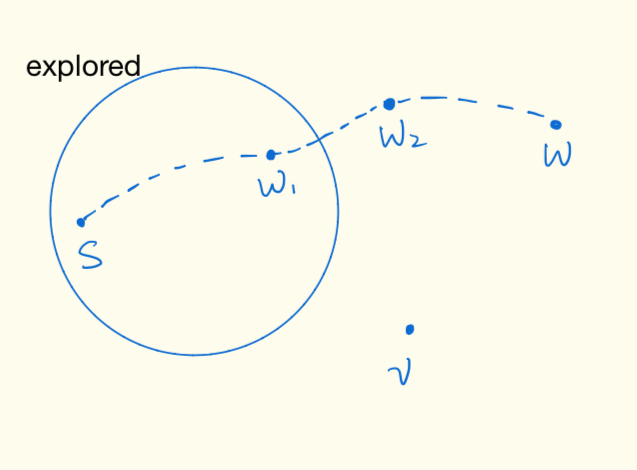
\includegraphics[scale = 0.35]{p1.png}
\end{center}

Denote the subpath from $s$ to $w_1$ in $p_w$ as $p(s, w_1)$, subpath $w_1$ to $w_2$ as $p(w_1, w_2)$, and subpath $w_2$ to $w$ as $p(w_2, w)$. Since $w_1$ is right before $w_2$ in $p_w$, then $length(p(w_1, w_2)) = weight(w_1, w_2)$. Then: 
\\\\
  \tab $\delta(w) = length(p_w) = length(\Delta(s, w_1)) + weight(w_1, w_2) + length(w_2, w)$
\\\\
Since all edge weights are positive, then: 
\\\\
  \tab $length(\Delta(s, w_1)) + weight(w_1, w_2) \leq \delta(w)$\\
  \tab i.e., $\delta(w_1) + weight(w_1, w_2) \leq \delta(w)$
\\\\
Since during the $(k+1)^{th}$ iteration, $w_1 \in explored$, then $w_1$ must be added into $explored$ with all neighbors of $w_1$ updated during the $i^{th}$ iteration for some $i < k+1$. Then based on our inductive hypothesis, $dist_{k+1}[w_1] = \delta(w_1)$. Since the value of $dist[w_1]$ remains unchanged after adding $w_1$ into $explored$, then $dist_i[w_1] = dist_{k+1}[w_1] = \delta(w_1)$. 
\\
Since $w_1$ is the node right before $w_2$ in $p_w$ during the $(k+1)^{th}$ iteration, then $dist_{k+1}[w_2] = dist_{i}[w_1] + weight(w_1, w_2) = \delta(w_1) + weight(w_1, w_2)$. Since $\delta(w_1) + weight(w_1, w_2) \leq \delta(w)$, then $dist_{k+1}[w_2] \leq \delta(w)$([2]).
\\
Combining [1] and [2], we have: 
\\\\
\ftab $\delta(w) < dist_{k+1}[v]$([1])\\
\ftab $dist_{k+1}[w_2] \leq \delta(w)$([2])
\\\\
Hence $dist_{k+1}[w_2] < dist_{k+2}[v]$([3]). 
\\
Based on our assumption, during the $(k+1)^{th}$ generation, $w_2 \notin explored$ and $v$ is selected by the algorithm, then we must have $dist_{k+1}[w_2] \geq dist_{k+1}[v]$, which contradicts with [3]. Hence by the principle of prove by contradiction, there does not exsist $w \in unexplored$, such that $\delta(v) > \delta(w)$. (1) holds for the $(k+1)^{th}$ iteration. 

(Proof below are still under construction)
\item $dist[v] = \delta(v)$
\\\\
Suppose $dist[v]$ is associates with path $p \in path(s, v)$ during the $k^{th}$ iteration, and assume the shortest path from $s$ to $v$ is some path $p' \in path(s, v)$ different than $p$, $length(p') = \delta(v) < dist[v]$([b]). Suppose $v'$ is the node just before $v$ in $p'$. 
\\\\
\ftab $\delta(v) = dist[v'] + weight(v', v)$ \\
\\\\
Since all edge weights are non-negative, then $dist[v'] < \delta(v)$. Based on (1), since $\delta(v) < \delta(w) \forall w \in unexplored$, then $v'$ must be in $explored$. Since $v'$ is in $explored$ and has an edge to $v$, then the algorithm must have compared $dist[v'] + weight(v', v)$ to the current $dist[v]$ and chose $dist[v]$. Hence it must be $dist[v'] + weight(v', v) \geq dist[v]$, i.e. $\delta(v) \geq dist[v]$, which contradicts with [b]. Hence by the principle of prove by contradiction, $p$ is the shortest path from $s$ to $v$, and that $dist[v] = \delta(v)$. 
\end{enumerate}
Since we proved both (1) and (2) for the $k^{th}$ iteration, forall $k \leq 1$, we have proved that Lemma (1) holds.
\end{proof}

\begin{proof}\textbf{Prove of Correctness}
\\\\
By applying Lemma (1) to the last iteration of the algorithm, we obtained that for all nodes $n$ in the explored list, $dist[n]$ is indeed the shortest path distance value from source $s$ to $n$, hence Dijkstra's algorithm indeed calculates the shortest path distance value from the source $s$ to each node $n \in g$. 
\end{proof}

%---------------------------------------------------------------------------------
% Low-Level Contribution
%---------------------------------------------------------------------------------

\section{Low-Level Contribution}



%----------------------------------------------------------------------------------------
% Discussion
%----------------------------------------------------------------------------------------

\section{Discussion}



%----------------------------------------------------------------------------------------
% Related Work
%----------------------------------------------------------------------------------------

\section{Related Work}



%----------------------------------------------------------------------------------------
% Conclusion
%----------------------------------------------------------------------------------------

\section{Conclusion}

%----------------------------------------------------------------------------------------
% Bibliography
%----------------------------------------------------------------------------------------
\newpage % Includes a new page

\pagenumbering{roman} % Changes page numbering to roman page numbers
%\bibliography{literature}

\bibliography{literature.bib} % Add the filename of your bibliography
\bibliographystyle{apsr} % Defines your bibliography style
[1] V. Klasen, "Verifying dijkstra's algorithm with key," in Diploma Thesis, Universitat Koblenz-Landau, 2010.%\url{https://kola.opus.hbz-nrw.de/opus45-kola/frontdoor/deliver/index/docId/420/file/DA_KLASEN.pdf}
\newline
[2] Bove, Ana, and Peter Dybjer. “Dependent Types at Work.” Language Engineering and Rigorous Software Development Lecture Notes in Computer Science, 2009, pp. 57–99., \url{doi:10.1007/978-3-642-03153-3_2}. %\url{http://www.cse.chalmers.se/~peterd/papers/DependentTypesAtWork.pdf}
\newline
[3] R. Mange and J. Kuhn, "Verifying dijkstra algorithm in jahob," 2007, student project, EPFL.%\url{https://lara.epfl.ch/w/_media/dijkstra.pdf} 
\newline
[4] Filliâtre, Jean-Christophe. “Toccata.” Dijkstra's Shortest Path Algorithm, \url{toccata.lri.fr/gallery/dijkstra.en.html}.%\url{http://toccata.lri.fr/gallery/dijkstra.en.html}
\newline
[5] “Why3.” Why3, May 2015, \url{why3.lri.fr/#provers}. %\url{http://why3.lri.fr/#provers}
\newline
%[6] \url{http://lara.epfl.ch/w/jahob_system}
[6] E. W. Dijkstra. A note on two problems in connexion with graphs. Numerische Mathematik, 1:269–271, 1959.
\newline 
[7] Richard E. Bellman. On a routing problem. Quarterly of Applied Mathematics, 16:87–90, 1958.
\newline
[8] A. Shimbel. Structure in communication nets. Polytechnic Press of the Poly- technic Institute of Brooklyn, page 199–203, 1955.
% For citing, please see this sheet: http://merkel.texture.rocks/Latex/natbib.php

%----------------------------------------------------------------------------------------
% Appendix
%----------------------------------------------------------------------------------------
\newpage % Includes a new page
\section*{Appendix} % Stars disable section numbers
% \appendix % Uncomment if you want to add an "automatic" appendix
\pagenumbering{Roman} % Changes page numbering to Roman page numbers


%----------------------------------------------------------------------------------------
% Declaration
%----------------------------------------------------------------------------------------
\newpage % Includes a page break
\thispagestyle{empty} % Leaves the page style empty (no page number, no header, no footer)
\section*{Statutory Declaration} % Stars disable section numbers

\vspace*{1in} % Adds extra space between two paragraphs


%\vspace*{1in} % Adds extra space

% % Add field for signature, date, and place
% \hfill \signature{} 


%---------------------------------------------------------------------------------

\end{document}
